% !TEX root = main.tex

\section{处理器}
\subsection{处理器概述}
计算机五大组成部分:[控制器+数据通路(运算器)]处理器、存储器、输入、输出
\begin{itemize}
	\item 操作元件:组合逻辑电路,所有操作元件都必须从状态元件接受输入,并并将输出写入状态元件
	\item 状态元件:时序逻辑电路,只有状态元件可以存储信息
\end{itemize}
\begin{definition}[寄存器组(Register File)]
包含
\begin{enumerate}
\item 两个读端口(组合逻辑):busA和busB读入地址,经过一个取数时间(AccessTime)后,两条线有效
\item 一个写端口(时序逻辑):写使能为1且时钟边沿到达
\end{enumerate}
要经过一个clk-to-Q(门闩延迟),输入信号在寄存器的输出端才有效
\end{definition}
一个时钟周期就是一个节拍


\subsection{数据通路的建立}
CPU执行指令主要分为两个阶段
\begin{enumerate}
	\item 取指阶段(公共操作):
	\begin{itemize}
		\item 取指令
		\item $PC\gets PC+\Delta=PC+4$
		\item 译码
	\end{itemize}
	\item 执行阶段:
	\begin{itemize}
		\item 主存地址运算
		\item 取操作数
		\item 算术逻辑运算
		\item 存结果
		\item 判断检测异常事件
		\item 若有异常,则自动切换到异常处理程序
		\item 检测是否有中断请求,有则转中断处理
	\end{itemize}
\end{enumerate}
\begin{figure}[htbp]
\centering
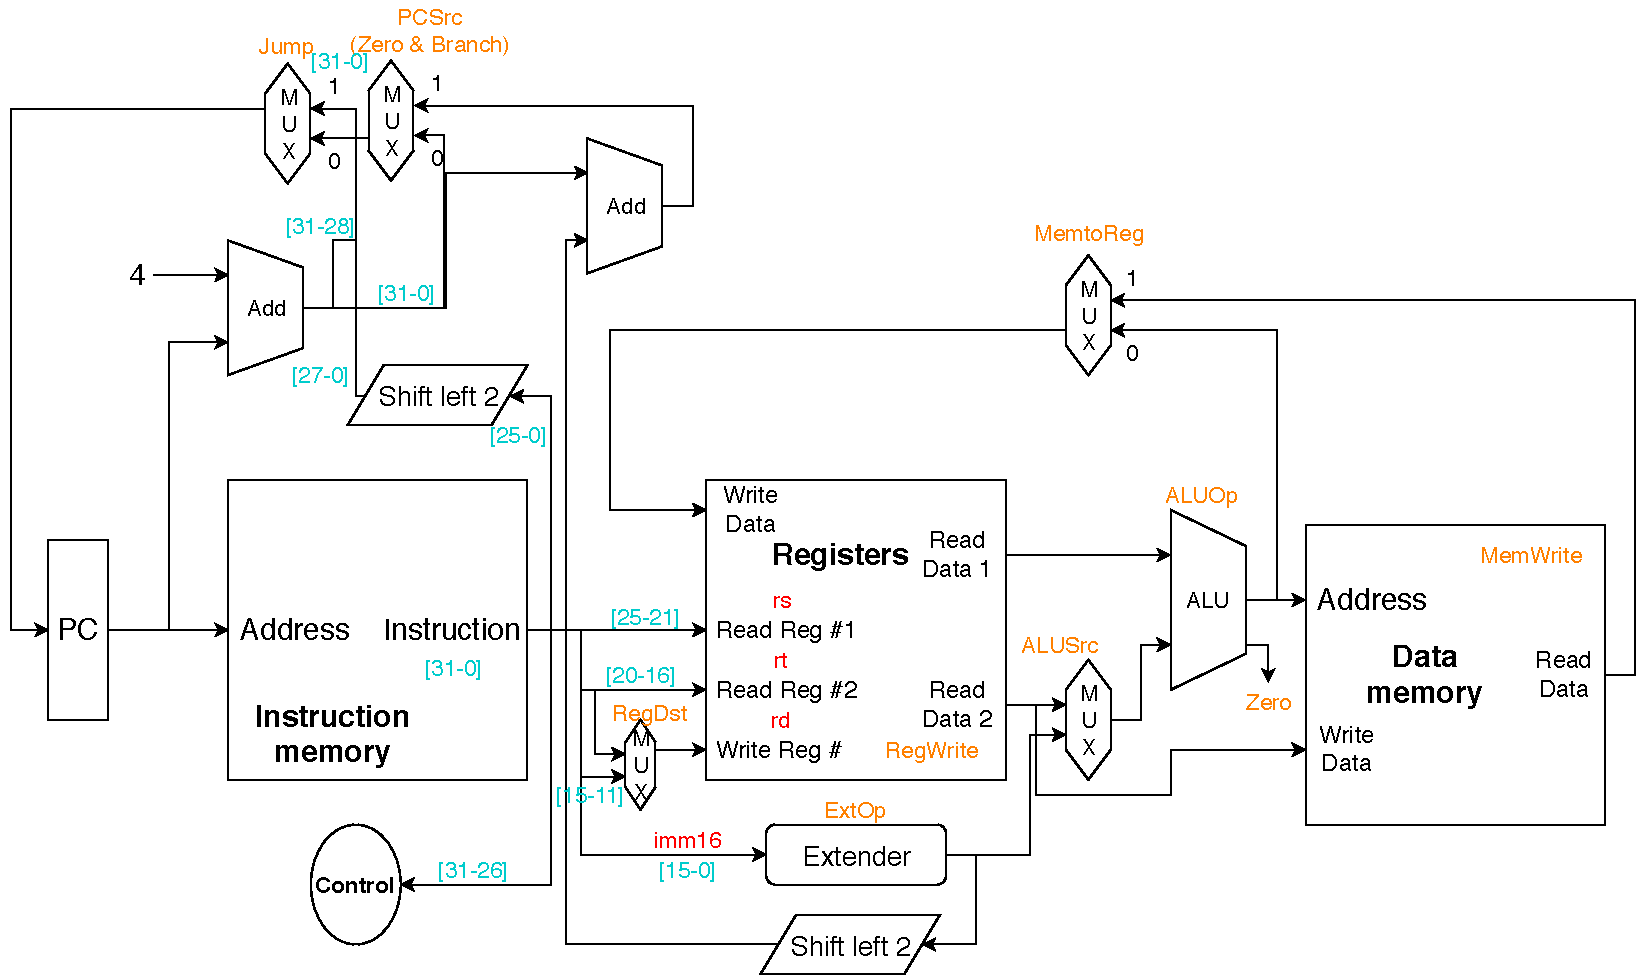
\includegraphics[width=\linewidth]{fig/Datapath_All.pdf}
\caption{MIPS基本数据通路}
\end{figure}
MIPS中三类基本指令:R-type、I-type、J-type\\
七条指令
\begin{enumerate}
	\item 加减 \verb'add/sub rd,rs,rt'
\begin{figure}[htbp]
\centering
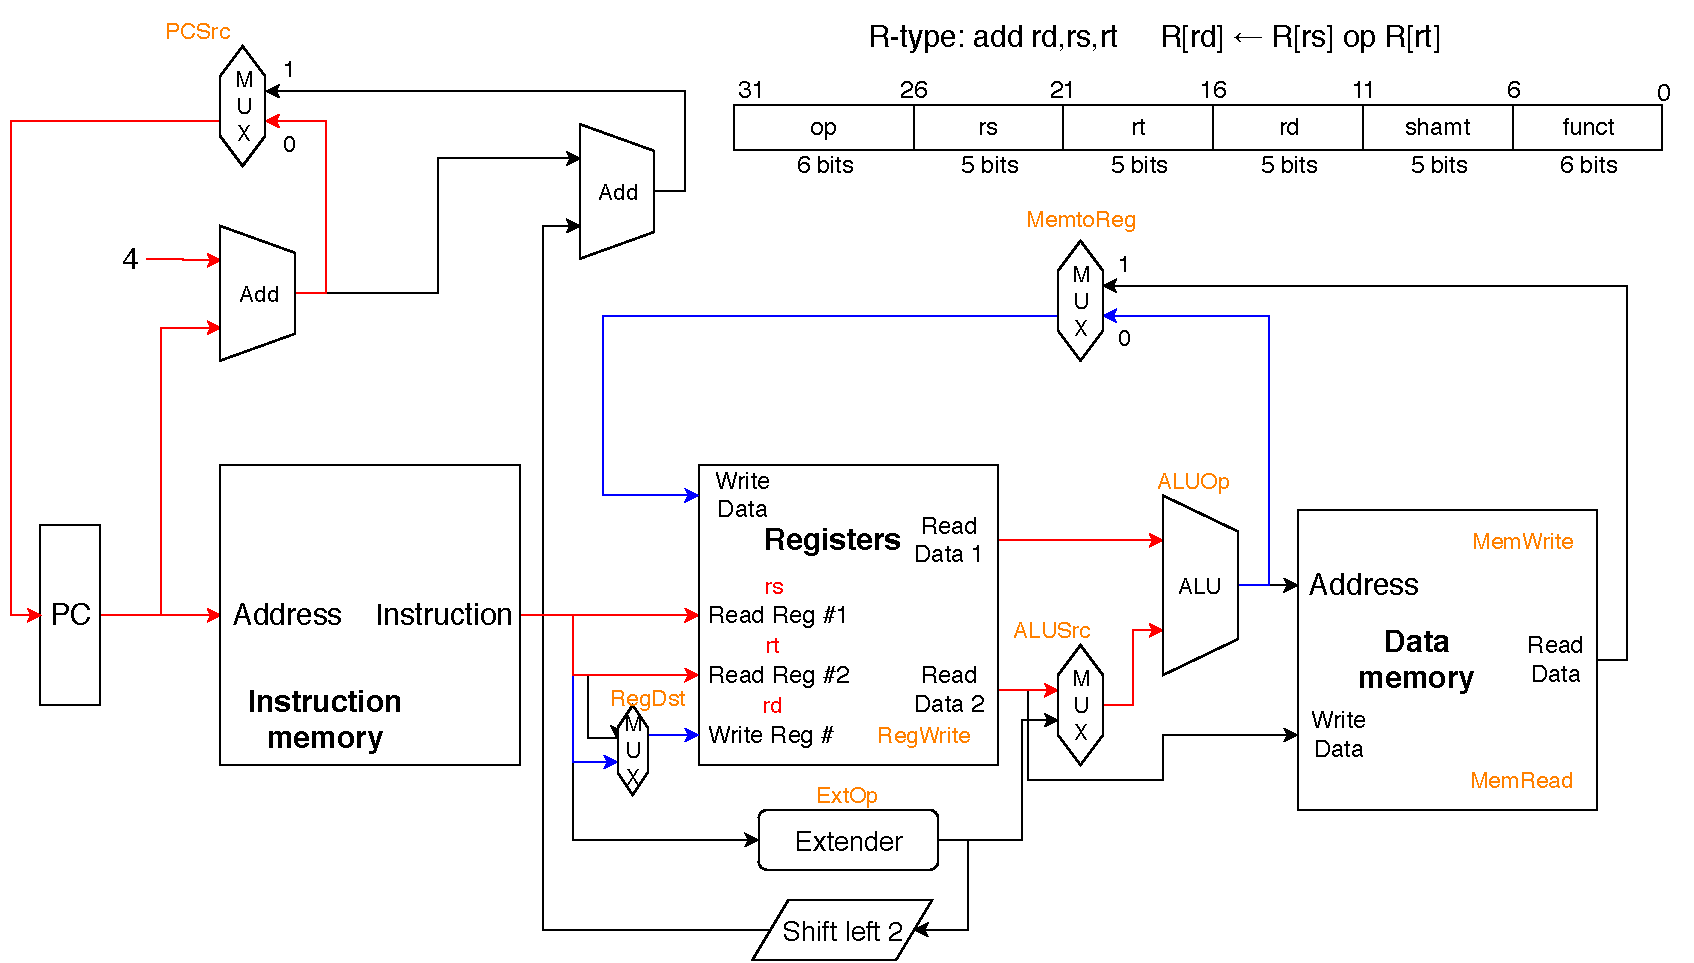
\includegraphics[width=\linewidth]{fig/Datapath_add.pdf}
\caption{add/sub通路}
\end{figure}
	\item 或立即数 \verb'ori rt,rs,imm16':零扩展
\begin{figure}[htbp]
\centering
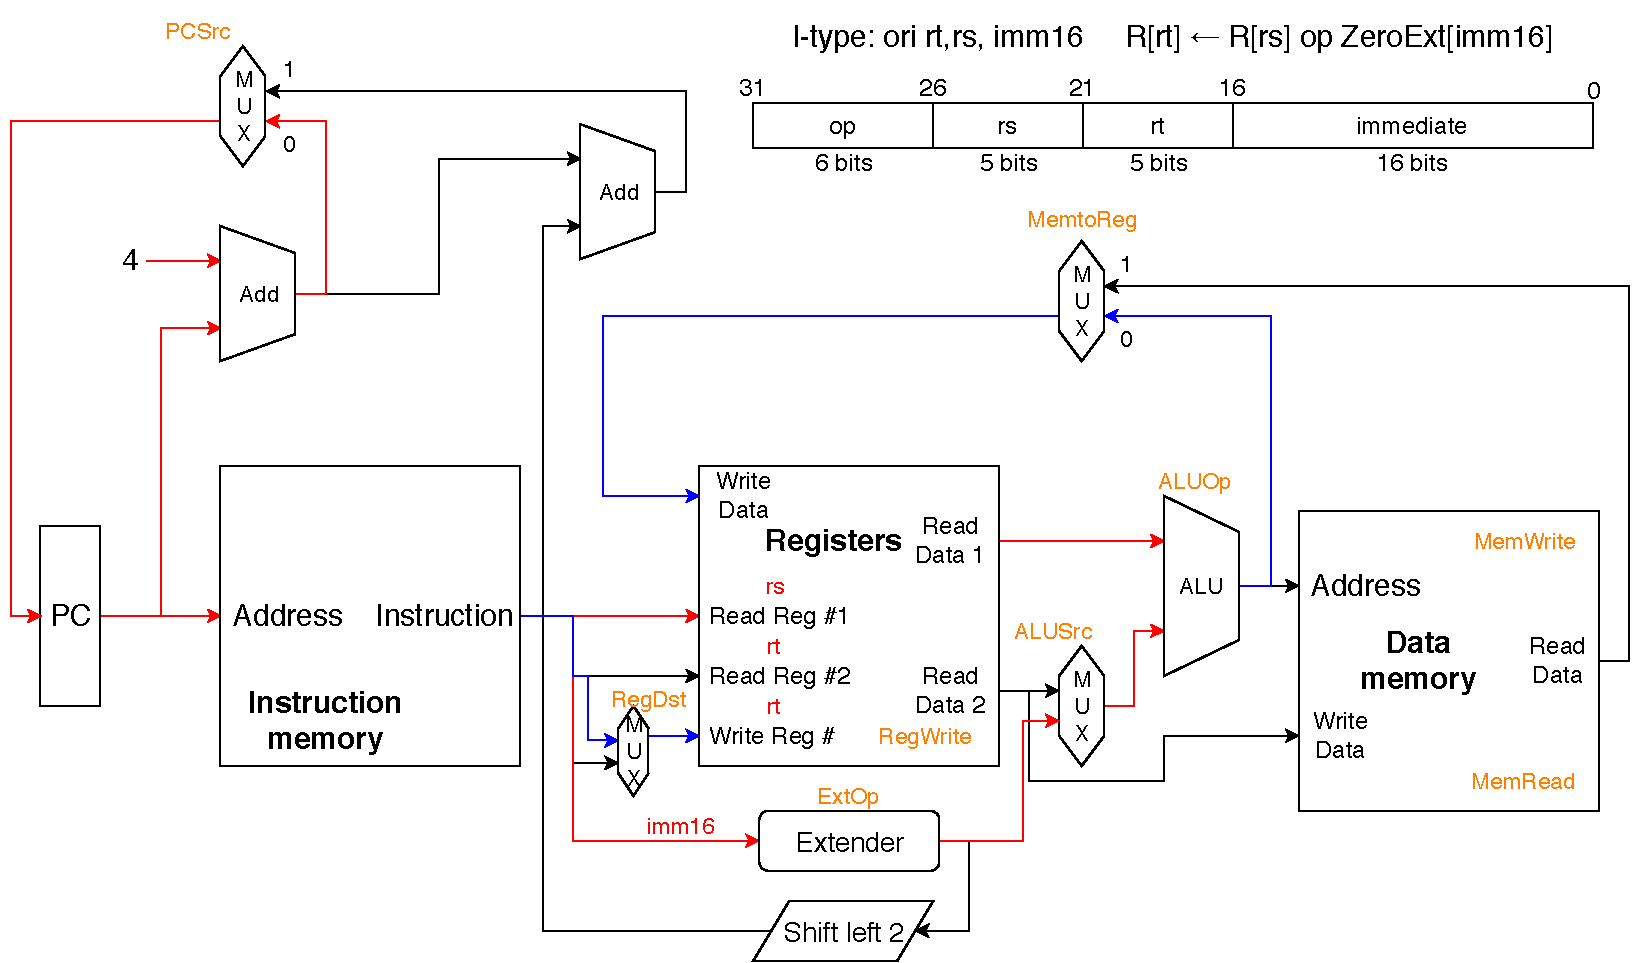
\includegraphics[width=\linewidth]{fig/Datapath_ori.pdf}
\caption{ori通路}
\end{figure}
	立即数需要零扩展(ZeroExt)为32位
	\item 存 \verb'lw rt,rs,imm16':符号扩展
\begin{figure}[htbp]
\centering
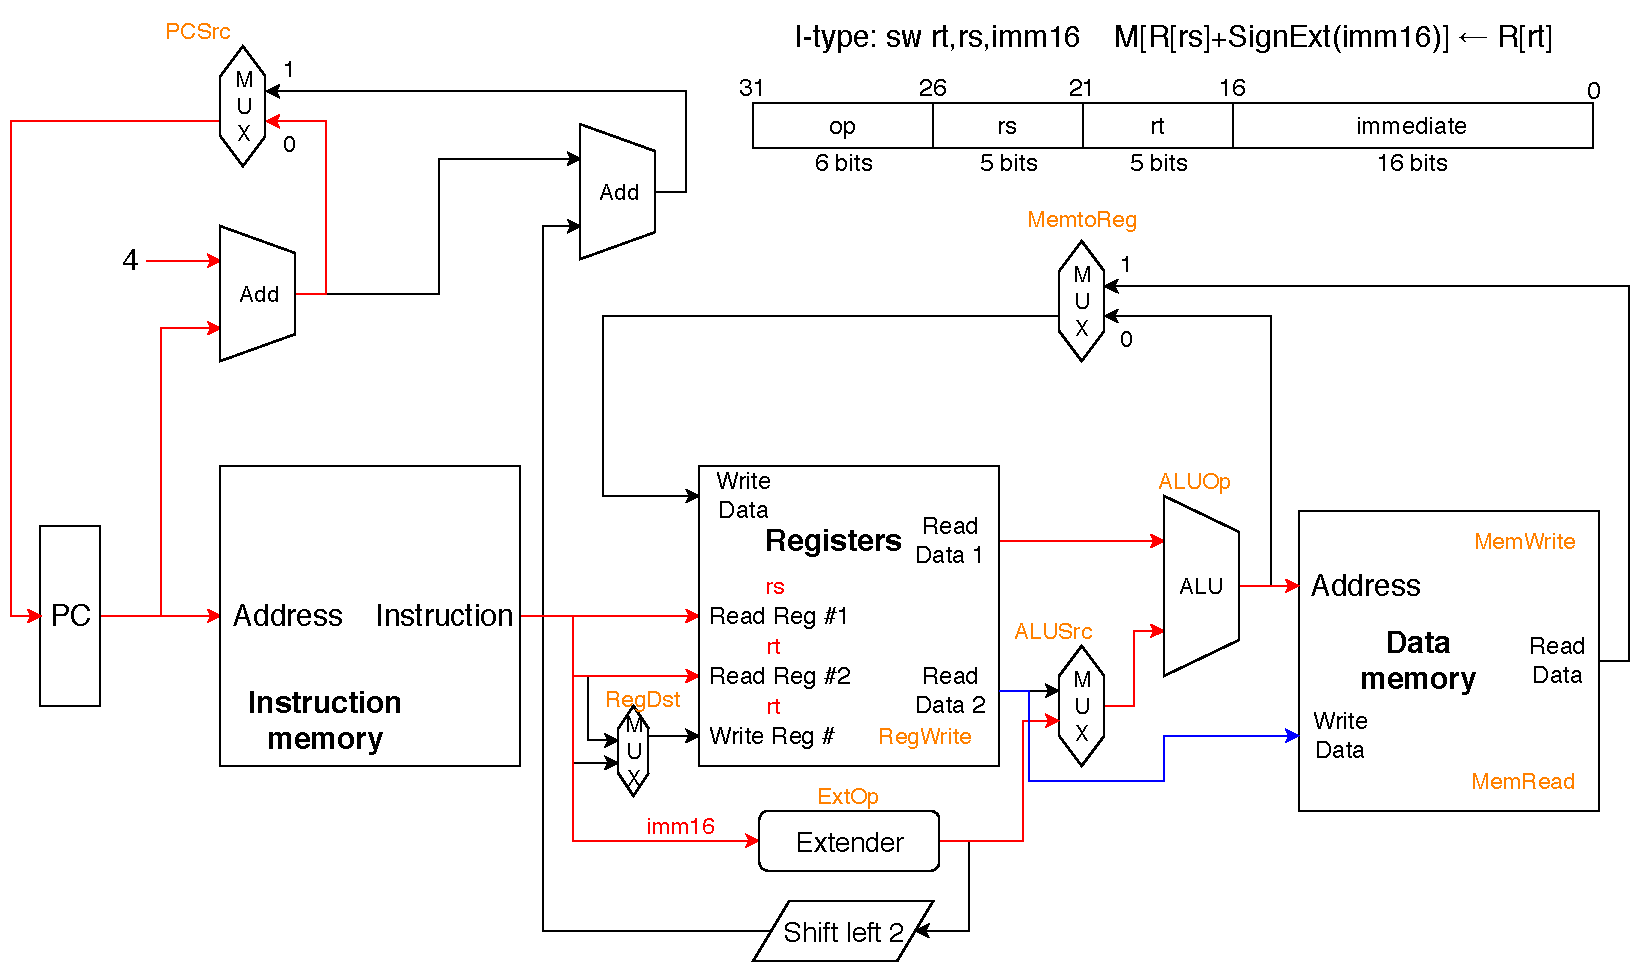
\includegraphics[width=\linewidth]{fig/Datapath_sw.pdf}
\caption{sw通路}
\end{figure}
	\item 取 \verb'sw rt,rs,imm16':符号扩展
\begin{figure}[htbp]
\centering
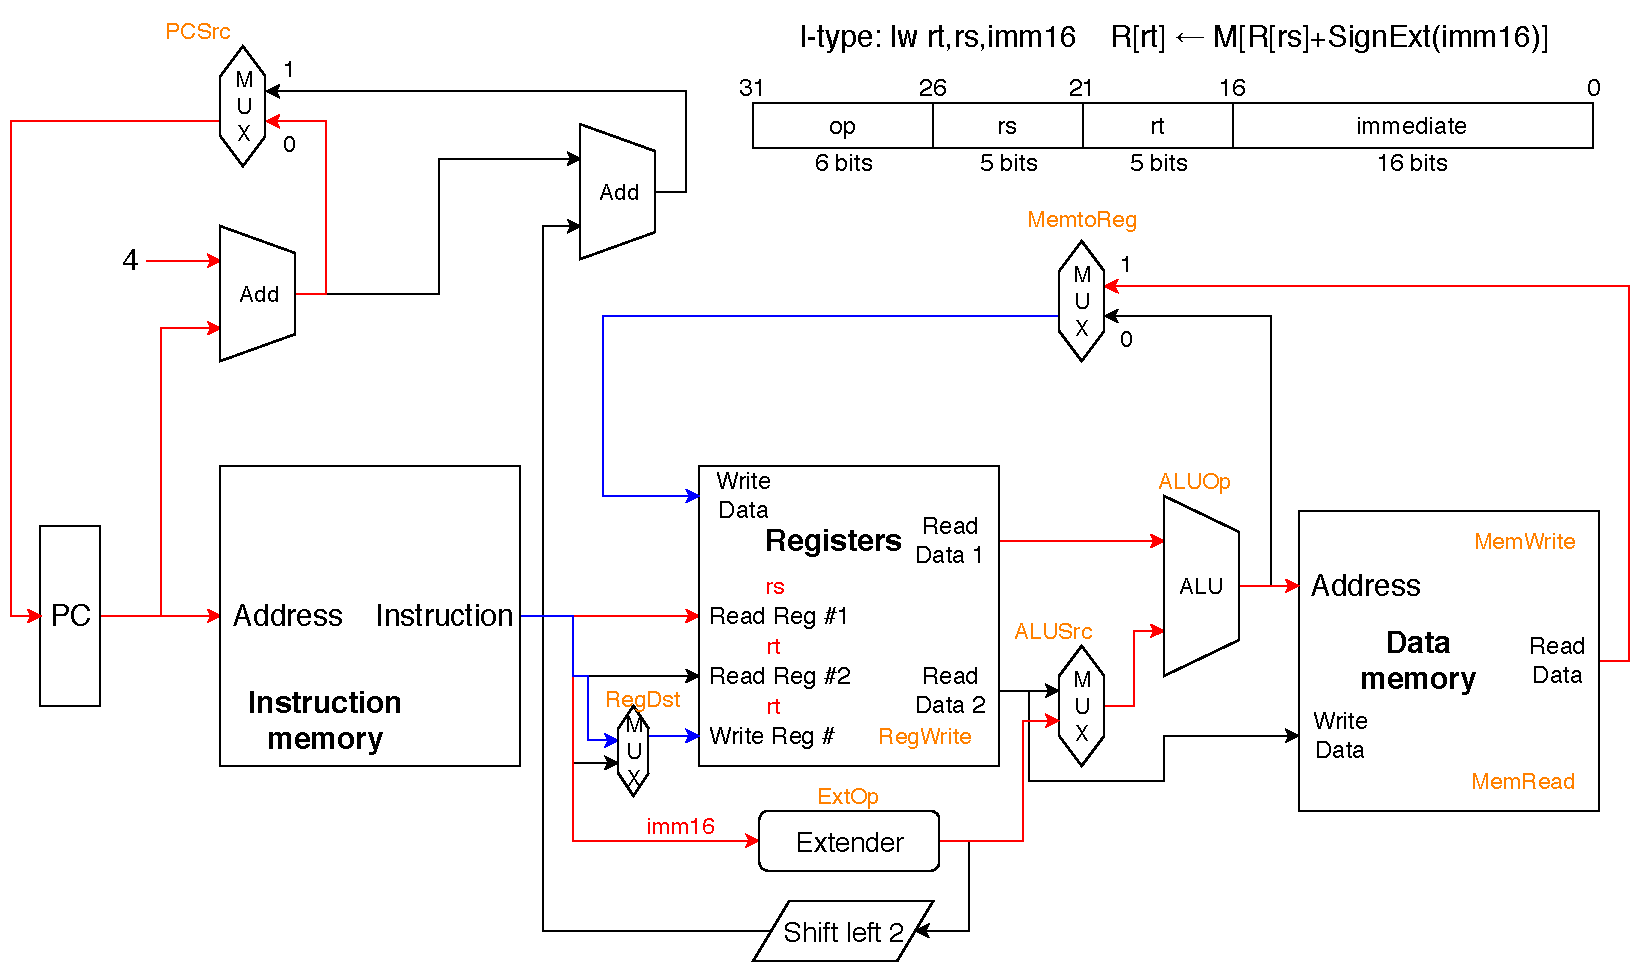
\includegraphics[width=\linewidth]{fig/Datapath_lw.pdf}
\caption{lw通路}
\end{figure}
	\item 分支 \verb'beq rs,rt,imm16':PC只需30位,因每次加4
\begin{figure}[htbp]
\centering
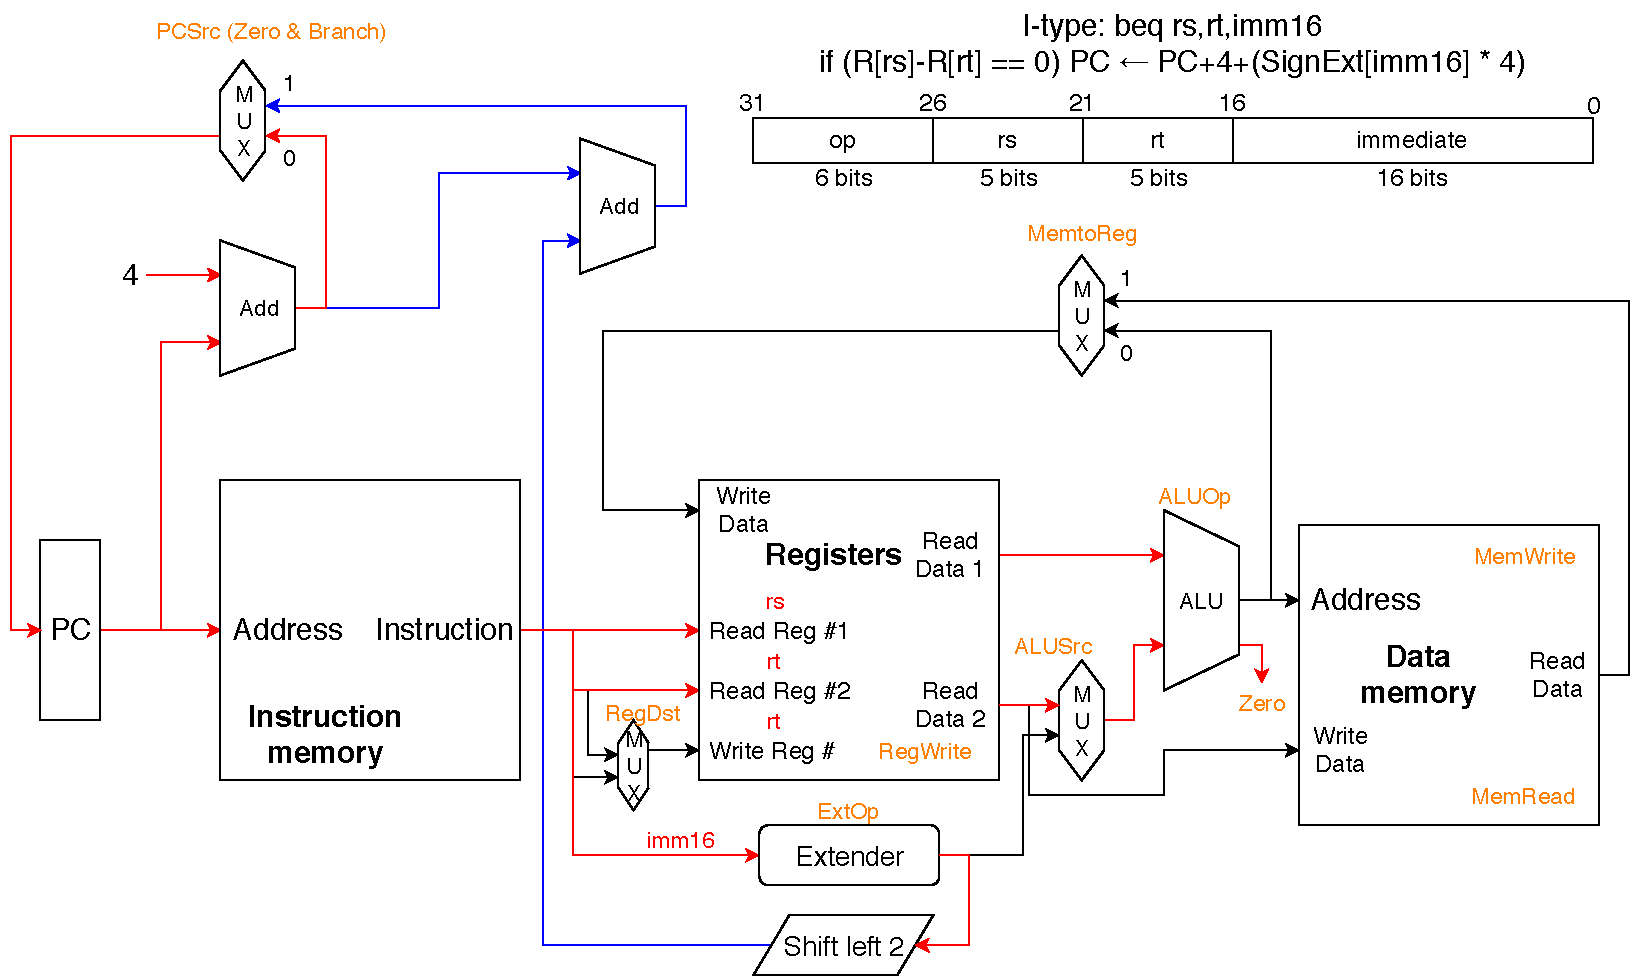
\includegraphics[width=\linewidth]{fig/Datapath_beq.pdf}
\caption{beq通路}
\end{figure}
	\item 跳转 \verb'j target':PC+4的高四位串接26位立即数然后左移2位
\begin{figure}[htbp]
\centering
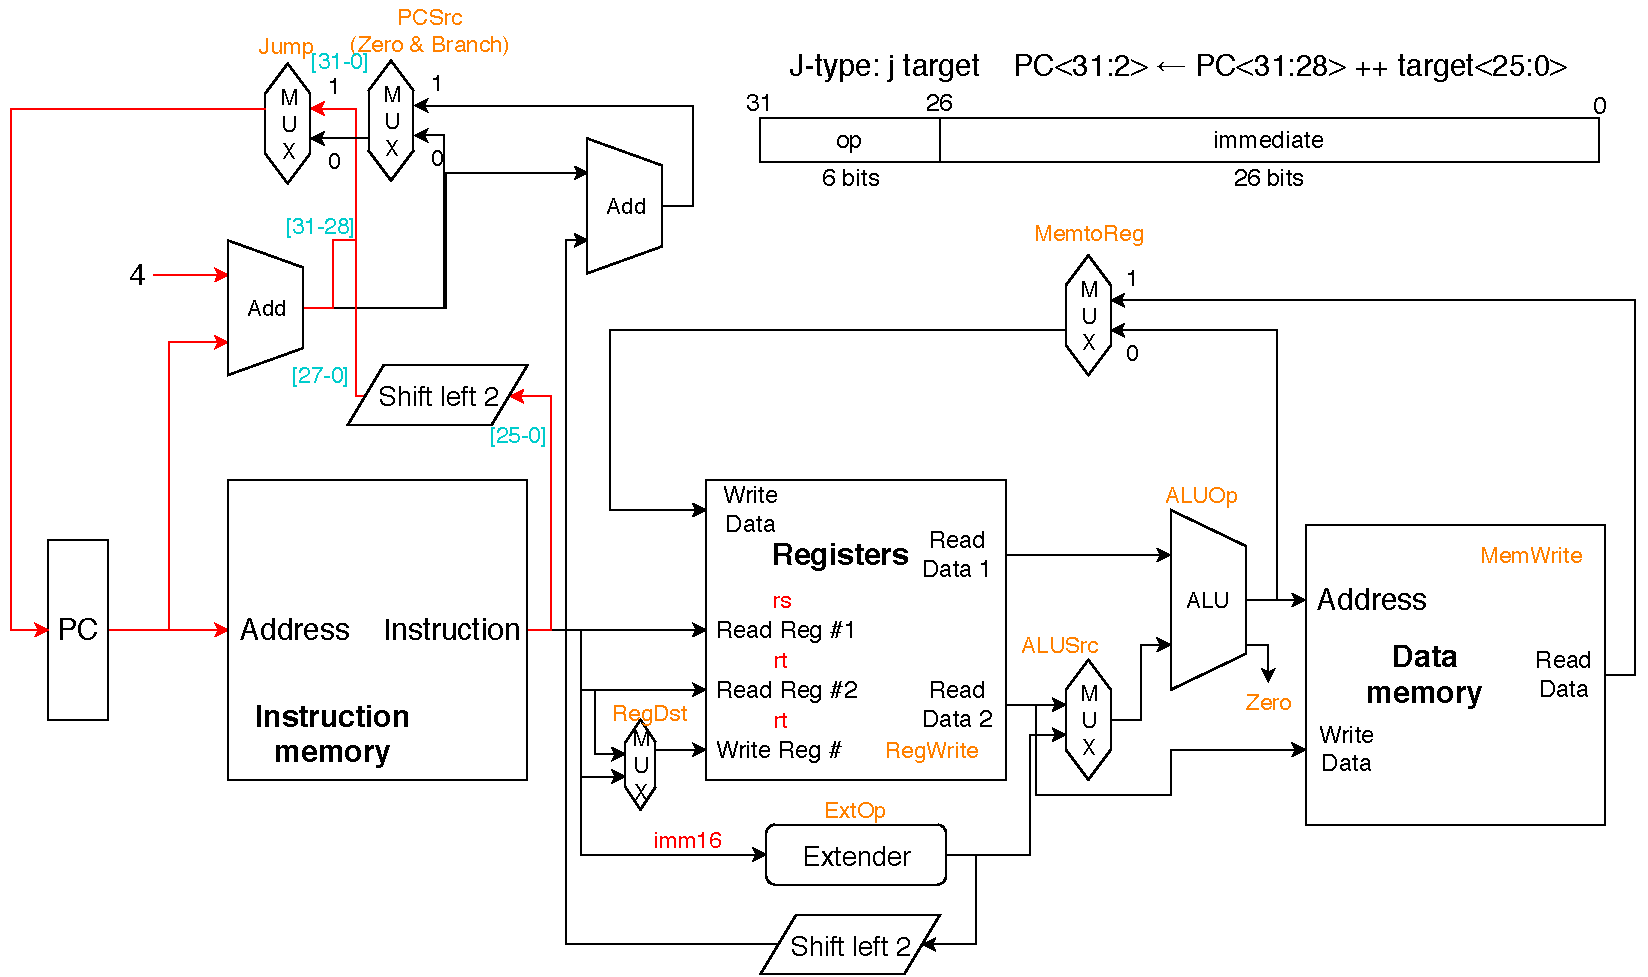
\includegraphics[width=\linewidth]{fig/Datapath_jump.pdf}
\caption{jump通路}
\end{figure}
\end{enumerate}

\subsection{多周期}
五个阶段:取指(IF)、译码(ID)、执行(EXE)、访存(MEM)、写回(WB)
\begin{itemize}
	\item 有限状态机:通过组合逻辑硬连线(PLA)实现
	\item 微程序:用ROM存放微程序实现
\end{itemize}

\subsection{流水线}
提升工作主频:\\
减少每个流水级执行时间$\to$减少每个流水级的任务量$\to$任务再分解$\to$增加流水线级数\\
副作用:
\begin{itemize}
	\item 寄存器开销(overhead):收益下降
	\item 非均匀延迟(Nonuniform delays):吞吐率受限于最慢栈的时间,但很难将ALU和存储器划分成更小的栈
\end{itemize}
单个任务执行时间没有缩短,但是总的吞吐率增加了\\
时钟周期等于最长阶段花费时间$t$,N条指令执行时间$(5+N-1)\times t$\\
利于流水线执行的指令集
\begin{itemize}
	\item 指令长度一致:简化取指和指令译码
	\item 指令格式少,且源寄存器位置相同:利于在指令未知时预取操作数
	\item 只有load/store指令才能访问存储器,利于减少操作步骤,规整流水线
	\item 数据和指令在内存中\textbf{对齐}存放,利于减少访存次数和流水线规整
\end{itemize}

\subsubsection{冒险(Harzard)}
\begin{itemize}
	\item 结构冒险/资源冲突:一个功能部件同时被多条指令使用产生,如Load和R-type同时要写回
	\begin{itemize}
		\item 通过加空操作(NOP)延迟写操作(每条指令都有五个阶段)
		\item 设置多个部件(比如多个端口、寄存器读写口分开),避免冲突
	\end{itemize}
	\item 控制冒险/分支冒险/转移冒险:在jump/beq之前已有几条指令被取出
	\begin{itemize}
		\item 静态分支预测:总是预测条件不满足,或加启发式规则
		\item 动态分支预测:根据历史情况进行调整(微型强化学习)
		\item 指令静态调度:编译优化指令顺序,实现分支延迟
	\end{itemize}
	\item 数据冒险/数据相关:写后读
	\begin{itemize}
		\item 转发(forwarding/bypassing):将数据从流水段寄存器中直接渠道ALU的输入端,如果在Data Memory读出则无法转发(Load-use数据冒险)
		\item 阻塞(stall):插入Bubble或插入NOP
		\item 静态指令调度:编译优化指令顺序,拉大具有数据冒险指令的距离,减少流水线可能产生的停顿(可以解决load-use);也即先把后面无关的操作调到前面来执行;或者说利用闲置资源先干后面的事情(乱序执行)% 只有在半并行(流水线)才会出现?
		\begin{figure}[htbp]
		\centering
		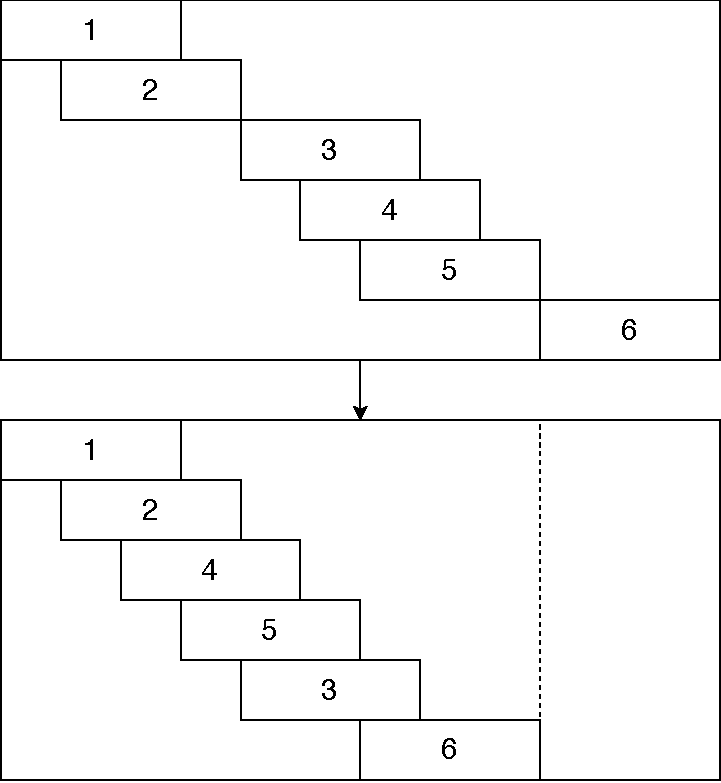
\includegraphics[width=0.3\linewidth]{fig/schedule.pdf}
		\caption{编译器调度}
		\end{figure}
	\end{itemize}
\end{itemize}